\documentclass[14pt,fleqn]{extarticle}
\RequirePackage{prepwell-eng}

\newcommand\dadt{\frac{da}{dt}}
\newcommand\dbdt{\frac{db}{dt}}
\newcommand\dcdt{\frac{dc}{dt}} 

\previewoff
\begin{document}
\begin{problem}
\statement
	

    $A, B$ and $C$ are three trains on three separate
    tracks (see figure). $T_2\parallel T_3$ and  $T_1\perp$ to both
    $T_2$ and $T_3$. Train $A$ has developed engine trouble 
    and is therefore being towards $M$ by $B$ using
    an iron-chain welded to the two trains. But 
    when $B$ is 30 meters from $N$ (and 40 meters 
    from $N$), it too develops engine trouble. So
    now, train $B$ is attached to train $C$ and is pulled
    towards $N$. If $C$ is moving at 3 m/s and the two
    chains ($AB$ and $BC$) are 50 m. long, 
    \underline{then how fast is $A$ moving}?
    
    \begin{center}
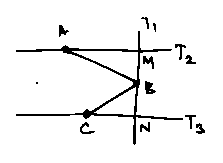
\includegraphics[scale=1.8]{333-A.eps}
\end{center}
    
\begin{step}
	\begin{options}
	
	\correct 
	
	The trains will move as shown below 
	\begin{center}
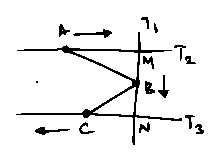
\includegraphics[scale=1.5]{333-B.eps}
\end{center}

	\incorrect 
	
	The trains will move as shown below 
	\begin{center}
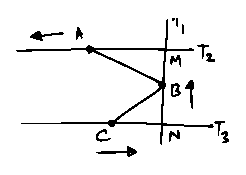
\includegraphics[scale=1.5]{333-C.eps}
\end{center}
	
	
	\end{options}
	\reason
	
      Train $A$ is being pulled towards $M$.
      Hence, $B$  must be moving towards $N$
      and train $C$ away from $N$ as shown below 
      
      \begin{center}
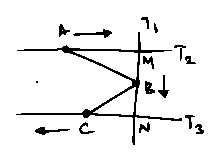
\includegraphics[scale=1.5]{333-B.eps}
\end{center}
      
\end{step}

\begin{step}
  \begin{options} 
     \correct 
       
     If $AM = a, BM = b$ and $CN = c$, then given that both the chains are $50$ m long 
     \[ \qquad\qquad \dadt = -\frac{4}{3}\cdot\dbdt \]  
     \incorrect
     
     If $AM = a, BM = b$ and $CN = c$, then given that both the chains are $50$ m long 
     \[ \qquad\qquad \dadt = -\frac{3}{4}\cdot\dbdt \]  
        
    \end{options} 
     \reason 
       
     \begin{align}
     a^2 + b^2 = AB^2 &= 50^2\\
     \therefore \underbrace{2a\cdot \dadt + 2b\cdot \dbdt}_{\text{Chain Rule}} &= 0 \\
     \implies \dadt &= -\frac{b}{a}\cdot \dbdt \\
     \text{But when }b &= 40\text{ m, then }\\
     a &= \sqrt{50^2 - 40^2} = 30 \\ 
     \therefore \dadt &= -\frac{40}{30}\cdot\dbdt \\
     &= -\frac{4}{3}\cdot\dbdt
\end{align}  
\end{step}

\begin{step}
  \begin{options} 
     \correct 
       
     Similarly, 
     \begin{align}
     \dbdt &= -\frac{4}{3}\cdot\dcdt \\
     \therefore \dadt &= -\frac{16}{3}\text{ m/s}
\end{align}  

Hence, Train $A$ is moving at $\frac{16}{3}$ m/s in the \underline{opposite} direction to $C$ when $B$ is $40$ meters from $M$
        
    \end{options} 
     \reason 
     
     When looking at trains $B$ and $C$, we can see that 
     \begin{align}
     &BN^2 + CN^2 = BC^2 = 50^2 \\
     &\implies (70-b)^2 + c^2 = 50^2 \\ 
     &\implies \underbrace{2\left(70-b \right)\cdot \frac{d}{dt} \left(70-b \right)
     + 2c\cdot\dcdt}_{\text{Chain Rule}} = 0 \\
     &\text{or } -2 \left(70-b \right)\cdot\dbdt + 2c\cdot\dcdt = 0 \\
     &\implies \dbdt = \frac{c}{70-b}\cdot\dcdt
\end{align}

But when $b = 40$, then 
\begin{align}
	BN = 70 -b &= 30 \\
	\text{and }c = \sqrt{50^2 - BN^2} &= 40
\end{align}
And therefore,
\begin{align}
\dbdt &= \frac{40}{30}\cdot\dcdt = \frac{4}{3}\cdot \left(3\text{ m/s} \right) = 4\text{ m/s} \\
\implies \dadt &= -\frac{4}{3}\cdot\dbdt = -\frac{4}{3}\cdot \left(4\text{ m/s} \right) \\
&= -\frac{16}{3}\text{ m/s}
\end{align}

The negative sign only means that $A$ is moving in the opposite direction to $C$

\end{step}

\end{problem}
\end{document}
